\documentclass[tikz,border=8pt]{standalone}
\usepackage{amsmath}
\usepackage{pgfplots}
\usepackage{xcolor}
\pgfplotsset{compat=1.18}

\definecolor{lineblue}{HTML}{2F6DB2}
\definecolor{lineorange}{HTML}{D97A2B}
\definecolor{linegreen}{HTML}{3D8B5A}
\definecolor{linegray}{HTML}{666666}

\begin{document}
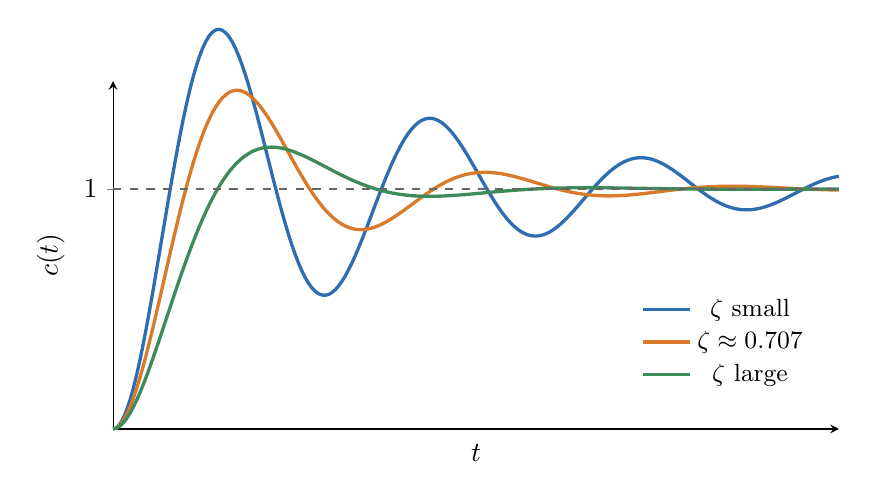
\begin{tikzpicture}
  \begin{axis}[
    width=10.8cm,
    height=6.0cm,
    xmin=0, xmax=8,
    ymin=0, ymax=1.45,
    axis lines=left,
    xlabel={$t$},
    ylabel={$c(t)$},
    xtick=\empty,
    ytick={1.0},
    yticklabels={$1$},
    legend style={draw=none, font=\small, at={(0.97,0.25)}, anchor=east},
    clip=false
  ]
    \addplot[line width=1.2pt, color=lineblue, samples=220, domain=0:8] {1 - exp(-0.35*x)*(cos(deg(2.7*x)) + 0.13*sin(deg(2.7*x)))};
    \addplot[line width=1.2pt, color=lineorange, samples=220, domain=0:8] {1 - exp(-0.65*x)*(cos(deg(2.3*x)) + 0.28*sin(deg(2.3*x)))};
    \addplot[line width=1.2pt, color=linegreen, samples=220, domain=0:8] {1 - exp(-1.0*x)*(cos(deg(1.8*x)) + 0.55*sin(deg(1.8*x)))};
    \addplot[dashed, color=linegray] coordinates {(0,1.0) (8,1.0)};
    \legend{$\zeta$ small,$\zeta\approx 0.707$,$\zeta$ large}
  \end{axis}
\end{tikzpicture}
\end{document}
